\documentclass[aspectratio=169]{beamer}
\usepackage[utf8]{inputenc}
\usepackage[T1]{fontenc}
\usepackage[brazil]{babel}
\usepackage{ragged2e}
\usepackage{booktabs}
\usepackage{verbatim}
\usepackage{gensymb}
\usepackage{multirow}
\usepackage{xcolor,colortbl}
\definecolor{verde}{rgb}{0,0.5,0}
\usepackage{listings}
\lstset{
  language=C++,
  basicstyle=\ttfamily\small,
  keywordstyle=\color{blue},
  stringstyle=\color{verde},
  commentstyle=\color{red},
  extendedchars=true,
  showspaces=false,
  showstringspaces=false,
%  numbers=left,
%  numberstyle=\tiny,
  breaklines=true,
  backgroundcolor=\color{green!10},
  breakautoindent=true,
  captionpos=b,
  xleftmargin=0pt
}
\newcommand\setItemnumber[1]{\setcounter{enumi}{\numexpr#1-1\relax}}

\usetheme{AnnArbor}
\usecolortheme{orchid}
\usefonttheme[onlymath]{serif}

\AtBeginSection[]{
  \begin{frame}
  \vfill
  \centering
  \begin{beamercolorbox}[sep=8pt,center,shadow=true,rounded=true]{title}
    \usebeamerfont{title}\insertsectionhead\par%
  \end{beamercolorbox}
  \vfill
  \end{frame}
}

\title[\sc{Template}]{Template}
\author[Roland Teodorowitsch]{Roland Teodorowitsch}
%\institute[LP2 - EC - PUCRS]{Laboratório de Programação II - Curso de Engenharia de Computação - PUCRS}
\institute[POO - EC - PUCRS]{Programação Orientada a Objetos - ECo - Curso de Engenharia de Computação - PUCRS}
\date{5 de junho de 2024}

\begin{document}
\justifying

%-------------------------------------------------------
\begin{frame}
	\titlepage
\end{frame}

%=======================================================
\section{Programação Genérica}

%-------------------------------------------------------
\begin{frame}\frametitle{Programação Genérica}
\begin{itemize}
	\item Os \textbf{genéricos} (ou \emph{\textbf{templates}}) são uma das mais poderosas maneiras de reuso de \emph{software}
	\begin{itemize}
		\item \textbf{Funções genéricas} e \textbf{classes genéricas} permitem que o programador especifique com apenas um segmento de código uma família de funções ou classes relacionadas (sobrecarregadas)
		\item Esta tecnica e chamada \textbf{programação genérica}
	\end{itemize}
\end{itemize}
\end{frame}

%-------------------------------------------------------
\begin{frame}\frametitle{Programação Genérica}
\begin{itemize}
	\item Por exemplo, é possível criar uma \textbf{função genérica} que ordene um vetor
	\begin{itemize}
		\item A linguagem se encarrega de criar especializações que tratarão vetores do tipo \texttt{int}, \texttt{float}, \texttt{string}, etc.
	\end{itemize}
	\item É possível tambem criar uma classe genérica para a estrutura de dados Pilha
	\begin{itemize}
		\item A linguagem se encarrega de criar as especializações para pilha de \texttt{int}, \texttt{float}, \texttt{string}, etc.
	\end{itemize}
	\item O \textbf{genérico} define o formato, a \textbf{especialização} e conteúdo
\end{itemize}
\end{frame}

%=======================================================
\section{Funções Genéricas}

%-------------------------------------------------------
\begin{frame}\frametitle{Funções Genéricas}
\begin{itemize}
	\item Funções sobrecarregadas normalmente realizam operações similares ou idênticas em diferentes tipos de dados
	\begin{itemize}
		\item Soma de \texttt{int} e \texttt{float}
		\item Se as operações são idênticas para diferentes tipos, elas podem ser expressas mais compacta e convenientemente atraves de \textbf{funções genéricas}
	\end{itemize}
	\item O programador escreve a definição da função genérica
	\begin{itemize}
		\item Baseado nos parâmetros explicitamente enviados ou inferidos a partir da chamada da função, o compilador gera as especializações para cada tipo de chamada
	\end{itemize}
\end{itemize}
\end{frame}

%-------------------------------------------------------
\begin{frame}[fragile]\frametitle{Funções Genéricas}
\begin{itemize}
	\item Uma definição de \textbf{função genérica} começa com a palavra \texttt{template} seguida de uma lista de parâmetros genéricos entre \texttt{\textless} e \texttt{\textgreater}
	\item Cada parâmetro deve ser precedido por \texttt{class} ou \texttt{typename}
	\begin{itemize}
		\item Especificam que os parâmetros serão de qualquer tipo primitivo
	\end{itemize}
	\item Exemplos:
\begin{lstlisting}[language=C++]
template <typename T>
template <class TipoElemento>
template <typename TipoBorda, typename TipoPreenchimento>
\end{lstlisting}
\end{itemize}
\end{frame}

%-------------------------------------------------------
\begin{frame}[fragile]\frametitle{Exemplo 1: definição}
\lstinputlisting[language=C,firstline=1,lastline=21,basicstyle=\ttfamily\tiny]{src/exemplo1.cpp}
\end{frame}

%-------------------------------------------------------
\begin{frame}[fragile]\frametitle{Exemplo 1: uso e resultado}
\begin{columns}
\begin{column}{0.65\linewidth}
\lstinputlisting[language=C,firstline=23,basicstyle=\ttfamily\tiny]{src/exemplo1.cpp}
\end{column}
\begin{column}{0.35\linewidth}
\lstinputlisting[language={},basicstyle=\ttfamily\scriptsize]{src/exemplo1.output}
\end{column}
\end{columns}
\end{frame}

%-------------------------------------------------------
\begin{frame}\frametitle{Funções Genéricas}
\begin{itemize}
	\item Quando o compilador detecta a chamada a \texttt{printArray()}, ele procura a definição da função
	\begin{itemize}
		\item Neste caso, a função genérica
		\item Ao comparar os tipos dos parâmetros, nota que há um tipo genérico
		\item Então, deduz qual deverá ser a substituição a ser feita:
		\begin{itemize}
			\item \texttt{T} por \texttt{int}
		\end{itemize}
		\item O compilador cria três especializações:
		\begin{itemize}
			\item \texttt{void printArray(const int *, int);}
			\item \texttt{void printArray(const double *, int);}
			\item \texttt{void printArray(const char *, int);}
		\end{itemize}
	\end{itemize}
\end{itemize}
\end{frame}

%=======================================================
\section{Classes Genéricas}

%-------------------------------------------------------
\begin{frame}\frametitle{Classes Genéricas}
\begin{itemize}
	\item Para se compreender o funcionamento da estrutura de dados \texttt{Pilha}, não importa o tipo dos dados empilhados/desempilhados
	\begin{itemize}
		\item No entanto, para implementar uma pilha, é necessário associá-la a um tipo
	\end{itemize}
	\item Esta é uma das grandes oportunidade de \textbf{reuso de \emph{software}}
	\item O ideal é descrever uma pilha genéricamente, assim como ela é entendida
	\item Instanciar versões específicas desta \textbf{classe genérica} fica por conta do compilador
\end{itemize}
\end{frame}


%-------------------------------------------------------
\begin{frame}\frametitle{Classes Genéricas}
\begin{itemize}
	\item \textbf{Classes Genéricas} (ou \textbf{Tipos Parametrizados}) requerem um ou mais parâmetros de tipo que especifiquem como customizá-las
	\begin{itemize}
		\item Gerando assim \textbf{especializações de classes genéricas}
	\end{itemize}
	\item O programador codifica apenas a definição da classe genérica
	\begin{itemize}
		\item A cada vez que uma especialização diferente for necessária, o compilador codifica a especialização
		\item Uma classe genérica \texttt{Pilha} vira uma coleção de classes especializadas:
		\begin{itemize}
			\item Pilha de \texttt{int}, \texttt{float}, \texttt{string}, frações, restaurantes, etc.
		\end{itemize}
	\end{itemize}
\end{itemize}
\end{frame}

%-------------------------------------------------------
\begin{frame}\frametitle{Classes Genéricas}
\begin{itemize}
	\item A definição de uma \textbf{classe genérica} é semelhante à definição de uma classe normal
	\begin{itemize}
		\item Antes da definição da classe, adiciona-se o cabeçalho:\\
		\texttt{template \textless{}typename T\textgreater}
		\item Em que o \texttt{T} representa o tipo que a classe manipula, passado como um parâmetro
		\begin{itemize}
			\item Na verdade, qualquer identificador serve, mas \texttt{T} é padrão
		\end{itemize}
		\item Em caso de tipos definidos pelo programador, deve-se tomar cuidados com a sobrecarga de operadores e também garantir a existência de pelo menos um construtor (o \emph{default})
	\end{itemize}
\end{itemize}
	\end{frame}

%-------------------------------------------------------
\begin{frame}[fragile]\frametitle{Exemplo 2: definição}
\lstinputlisting[language=C,firstline=1,lastline=27,basicstyle=\ttfamily\tiny]{src/exemplo2.cpp}
\end{frame}

%-------------------------------------------------------
\begin{frame}[fragile]\frametitle{Exemplo 2: implementação}
\lstinputlisting[language=C,firstline=29,lastline=55,basicstyle=\ttfamily\tiny]{src/exemplo2.cpp}
\end{frame}

%-------------------------------------------------------
\begin{frame}[fragile]\frametitle{Exemplo 2: uso e resultado}
\begin{columns}
\begin{column}{0.65\linewidth}
\lstinputlisting[language=C,firstline=57,basicstyle=\ttfamily\tiny]{src/exemplo2.cpp}
\end{column}
\begin{column}{0.35\linewidth}
\lstinputlisting[language={},basicstyle=\ttfamily\scriptsize]{src/exemplo2.output}
\end{column}
\end{columns}
\end{frame}

%-------------------------------------------------------
\begin{frame}\frametitle{Classes Genéricas}
\begin{itemize}
	\item Os membros de uma \textbf{classe genérica} são \textbf{funções genéricas}
	\begin{itemize}
		\item As definições que aparecem fora da classe devem ser precedidas pelo cabeçalho:\\
		\texttt{template \textless{}typename T\textgreater}
		\item O operador de escopo utiliza o nome da \textbf{classe genérica}:\\
		\texttt{Stack \textless{}T\textgreater}
		\item Na implementação, os elementos da pilha aparecem genéricamente como sendo do tipo \texttt{T}
	\end{itemize}
\end{itemize}
\end{frame}

%-------------------------------------------------------
\begin{frame}\frametitle{Classes Gené	ricas}
\begin{itemize}
	\item Para instanciar um objeto de uma \textbf{classe genérica}, é preciso informar qual tipo deve ser associado à classe
	\begin{itemize}
		\item No exemplo, foram declarados dois objetos, associando os tipos \texttt{double} e \texttt{int}
		\item O compilador substituirá o tipo do \texttt{T} da definição da classe pelo tipo informado, e criará uma nova codificação da classe
		\item Note que o código na função principal é idêntico para as duas pilhas criadas
	\end{itemize}
\end{itemize}
\end{frame}

%=======================================================
\section{Outros Parâmetros e Parâmetros Padronizados}

%-------------------------------------------------------
\begin{frame}[fragile]\frametitle{Outros Parâmetros}
\begin{itemize}
	\item A \textbf{classe genérica} do exemplo anterior recebia apenas um parâmetro, que representava um tipo
	\begin{itemize}
		\item No entanto, uma classe pode receber mais que um parâmetro
		\item O parâmetro não precisa necessariamente representar um tipo
		\item Por exemplo, uma \textbf{classe genérica} poderia receber também um inteiro que representasse o tamanho da pilha
\begin{lstlisting}[language=C++]
template <typename T, int elementos>
class Stack {
\end{lstlisting}
	\end{itemize}
\end{itemize}
\end{frame}

%-------------------------------------------------------
\begin{frame}[fragile]\frametitle{Parâmetros Padronizados}
\begin{itemize}
	\item Outra possibilidade é definir valores padrão para os parâmetros de uma \textbf{classe genérica}:
\begin{lstlisting}[language=C++]
template <typename T = int>
class Stack {
\end{lstlisting}
	\item No exemplo acima, caso um tipo não seja especificado, será criada uma pilha de inteiros pela chamada abaixo:
\begin{lstlisting}[language=C++]
Stack<> intStack(5);
\end{lstlisting}
	\item Parâmetros padronizados devem ser definidos mais à direita na lista de parâmetros
	\begin{itemize}
		\item Quando se instancia uma classe com um ou mais parâmetros padronizados, se um parâmetro omitido não é o mais à direita, então todos os parâmetros depois dele também devem ser omitidos
	\end{itemize}
\end{itemize}
\end{frame}

%=======================================================
\section{Classes Genéricas e Herança}

%-------------------------------------------------------
\begin{frame}\frametitle{Classes Genéricas e Herança}
\begin{itemize}
	\item Os conceitos associados à \textbf{herança} podem ser utilizados em \textbf{classes genéricas}
	\begin{itemize}
		\item Além de gerar classes, é possível gerar hierarquias de classes com templates
		\item Cada hieraquia é parametrizada
		\item \textbf{Funções virtuais} são permitidas na hierarquia, ou seja, é possível usar \textbf{polimorfismo}
		\item Pode-se ter também \textbf{classes template abstratas}, etc.
	\end{itemize}
\end{itemize}
\end{frame}

%-------------------------------------------------------
\begin{frame}[fragile]\frametitle{Exemplo 3}
\begin{columns}
\begin{column}{0.6\linewidth}
\lstinputlisting[language=C,firstline=1,lastline=27,basicstyle=\ttfamily\tiny]{src/exemplo3.cpp}
\end{column}
\begin{column}{0.4\linewidth}
\lstinputlisting[language=C,firstline=29,basicstyle=\ttfamily\tiny]{src/exemplo3.cpp}
\end{column}
\end{columns}
\end{frame}

%=======================================================
\section{Considerações sobre o uso de \texttt{const}}

%-------------------------------------------------------
\begin{frame}[fragile]\frametitle{Considerações sobre o uso de \texttt{const}}
\begin{columns}
\begin{column}{0.5\linewidth}
\begin{itemize}
	\item Observe o seguinte trecho de código, que envolve uma variável e um ponteiro
\lstinputlisting[language=C,firstline=13,lastline=26,basicstyle=\ttfamily\tiny]{src/const.cpp}
\end{itemize}
\end{column}
\begin{column}{0.5\linewidth}
\begin{itemize}
	\item É possível ter um ponteiro variável apontando para um conteúdo constante
\lstinputlisting[language=C,firstline=30,lastline=43,basicstyle=\ttfamily\tiny]{src/const.cpp}
\end{itemize}
\end{column}
\end{columns}
\end{frame}

%-------------------------------------------------------
\begin{frame}[fragile]\frametitle{Considerações sobre o uso de \texttt{const}}
\begin{columns}
\begin{column}{0.5\linewidth}
\begin{itemize}
	\item Também seria possível ter um ponteiro constante apontando para um conteúdo variável
\lstinputlisting[language=C,firstline=47,lastline=58,basicstyle=\ttfamily\tiny]{src/const.cpp}
\end{itemize}
\end{column}
\begin{column}{0.5\linewidth}
\begin{itemize}
	\item Por fim, seria possível ter um ponteiro constante apontando para um conteúdo constante
\lstinputlisting[language=C,firstline=62,lastline=73,basicstyle=\ttfamily\tiny]{src/const.cpp}
\end{itemize}
\end{column}
\end{columns}
\end{frame}

%=======================================================
\section{Lista de Exercícios}

%-------------------------------------------------------
\begin{frame}[fragile]\frametitle{Exercício 1}
\begin{enumerate}
	\setItemnumber{1}
	\item A função abaixo só ordena arranjos de elementos do tipo \texttt{int}.
	\begin{itemize}
		\item Escreva a função genérica correspondente;
		\item Escreva um programa que utiliza a função genérica.
	\end{itemize}
\begin{lstlisting}[language=C++,basicstyle=\ttfamily\scriptsize]
void selection_sort(int v[], int N){
  for(int i=0; i<N-1; i++){
     int menor = i;
     for(int j=i+1; j<N; j++)
        if (v[j]<v[menor]) menor = j;
     if (menor!=i) {
        int aux = v[i];
        v[i] = v[menor];
        v[menor] = aux;
     }
  }
}
\end{lstlisting}
\end{enumerate}
\end{frame}

%-------------------------------------------------------
\begin{frame}[fragile]\frametitle{Exercício 2}
\begin{enumerate}
	\setItemnumber{2}
	\item Modifique a classe \texttt{ListaLinkSinal} do exercício da aula sobre ``Estruturas Encadeadas'' para que ao invés de armazenar números inteiros (atributo \texttt{Dado}), ela possa armazenar um \texttt{string} ou um número real.
\begin{figure}[h]
	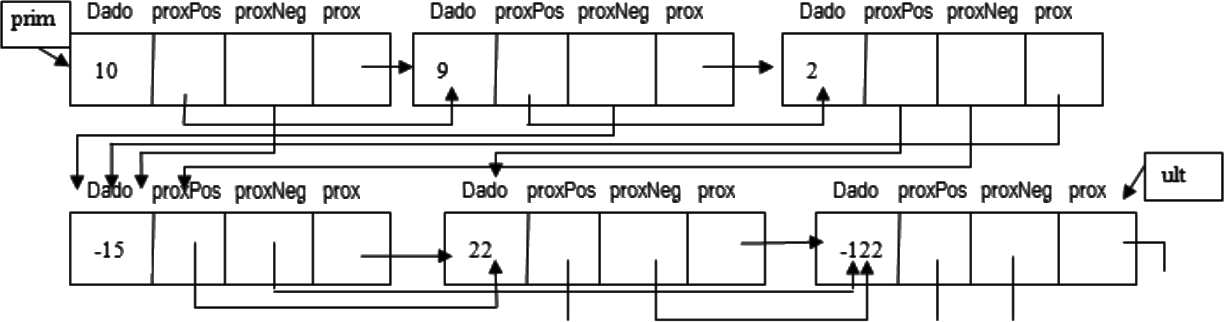
\includegraphics[height=0.35\paperheight]{pucrs-ec-poo-unidade_15-templates-laminas-estrutura_encadeada.png}
\end{figure}
\end{enumerate}
\end{frame}

%=======================================================
\section{Creditos}

%-------------------------------------------------------
\begin{frame}\frametitle{Creditos}
\begin{itemize}
	\item Estas lâminas contêm trechos de materiais disponibilizados pelos professores Rafael Garibotti e Edson Moreno.
\end{itemize}
\end{frame}

%=======================================================
\section{Soluções}

%-------------------------------------------------------
\begin{frame}\frametitle{Exercício 1}
\begin{columns}
\begin{column}{0.5\linewidth}
\lstinputlisting[language=C,firstline=1,lastline=17,basicstyle=\ttfamily\tiny]{src/exercicio01.cpp}
\end{column}
\begin{column}{0.5\linewidth}
\lstinputlisting[language=C,firstline=19,basicstyle=\ttfamily\tiny]{src/exercicio01.cpp}
\end{column}
\end{columns}
\end{frame}

%-------------------------------------------------------
\end{document}

